\newcommand{\PublicDocument}{\equal{1}{1}}

% Sample file using carp.cls
\documentclass{carp}

\usepackage[english]{babel}

\usepackage{amsmath}
\usepackage{mdwlist}
\usepackage{paralist}
\usepackage{amsfonts}
\usepackage{textcomp} % Used for syntax highlighting.
\usepackage{listings}
\usepackage{subcaption}

\usepackage{todonotes}
\usepackage{multicol}
% This gives syntax highlighting in the python environment
\renewcommand{\lstlistlistingname}{Code Listings}
\renewcommand{\lstlistingname}{Code Listing}

\renewcommand{\todo}[1]{}

\definecolor{gray}{gray}{0.5}
\definecolor{key}{rgb}{0,0.5,0}

% Document title
\title{
\ifthenelse{\PublicDocument}
{PENCIL 1.0 Language Specification}
{D3.5: Final PENCIL Language Specification}
}

% Document type (one of MD, TR, D, P)
\ifthenelse{\PublicDocument}{\type{TR}}{\type{D}}
% MD: management document
% TR: technical report
% D:  deliverable
% P:  published paper

% Document distribution (one of PU, PP, RE, CO)
\ifthenelse{\PublicDocument}{\distribution{PU}}{\distribution{PP}}
% PU: Public
% PP: Restricted to other programme participants (including commission services);
% RE: restricted to a group specified by the consortium (including the commission services);
% CO: confidential, only for members of the consortium (including the commission services).

% Name of editor
\editor{J.\ Absar (ARM)}

% Editing Partner, responsible for document (one of ICL, ENS, ARM, REAL, RWTHA, MONO, UT, RIGHT)
\epartner{ENS}

% Either a list of partners or a list of persons
\contributors{ARM, ENS}

% Local 3-digit number assigned by partner
\localnumber{004}

% Version number
\ifthenelse{\PublicDocument}{\versionnumber{v0.9}}{\versionnumber{v1.0}}

% Document code: one of
%Contract Change Notice	CN
%Contract	CO
%Change Request	CR
%Configuration Status List	CS
%Critical Items List	CI
%Design Document 	DD
%Dispatch Note	DN
%Data Package	DP
%Drawing	DW
%Interface Control Document	ID
%List	LI
%Minutes of Meeting	MM
%Memorandum	MO
%Non-Conformance Report	NC
%Plan	PL
%Progress Report	PR
%Presentation	PT
%Review Item Discrepancy	RD
%Report	RP
%Request for Waiver	RW
%Software Requirements Document	SR
%Statement of Work	SW
%Technical Note	TN
%Test Procedure	TP
%Test Report	TR
%Test Specification	TS
%User Manual	UM
\documentcode{RP}

% Names of authors/contributors

\author{R.\ Baghdadi$^1$, A.\ Cohen$^1$, T.\ Grosser$^1$, S.\ Verdoolaege$^1$ \\
  J.\ Absar$^2$, S.\ v.\ Haastregt$^2$, A.\ Kravets$^2$, A.\ Lokhmotov$^2$ \\
  J.\ Ketema$^3$, A.\ Donaldson$^3$}

% .... and their addresses (design this yourself)
\address{$^1$ENS, $^2$ARM, $^3$ICL}

% Contributing workpackages (sublist of WP1, WP1, WP2, WP3, WP4, WP5, WP6, WP7, WP8)
\workpackages{WP3}

% Date of delivery to the EC
\preparationdate{}
\duedate{30 April 2014}
\ecdate{1 Feb 2015}

\reviewers{ICL}

% Abstract (should not exceed 10 lines)
%\abstract{
%}

% Revision History: each line should have the following format
% Date & Version & Author & Modification \nl
% Please separate line by the command \nl which adds the needed horizontal line

\revhistory{
2015-02-01 & 1.0 & ENS & First Public Version\nl
}

\approvals{
Workpackage Leader & A.\ Lokhmotov & ARM & 2014-05-06 \nl
Project Manager & A.F.\ Donaldson & ICL & 2013-05-06 \nl
}

% Actual document starts here %%%%%%%%%%%%%%%%%%%%%%%%%%%%%%%%%%%%%%%%%%%%%%%%%%%%%%%%%%

\def\OPTL{\textrm{$[$}}
\def\OPTR{\textrm{$]$}}

\definecolor{lightbackground}{rgb}{.98,.98,.97}
\definecolor{darkgray}{rgb}{.3,.3,.3}
\definecolor{darkred}{rgb}{.6,0,0}
\definecolor{darkgreen}{rgb}{0,.6,0}
\definecolor{darkblue}{rgb}{0,0,.6}
\usepackage{listings}
\lstdefinelanguage{pencil}{%
  %% Definition du langage
  %% List of keywords
  keywords={[1]},%for,do,while,if,else,break,continue,return
  keywords={[2]struct,union,enum,typedef,volatile,%
    signed,unsigned,sizeof,typeof,inline,noinline,%
    void,char,short,long,int,float,double,boolean,size_t},
  keywords={[3]pragma,pencil,independent,ivdep,reduction,access, region},
  keywords={[4],__attribute__,%
    pencil_access,__pencil_kill,KILL,__pencil_assume,ASSUME,__pencil_assert,%
    __pencil_maybe,MAYBE,__pencil_use,USE,__pencil_def,DEF,MAY_DEF,%
    PENCIL,__pencil_access,ACCESS,CONST,pencil_heap,HEAP,const,restrict,static},
  %emph={main,producer,consumer,master,selector,compute,hscan,sync_av},
  %% List of abbreviations
  % literate={<=}{{$\leq$}}1 {>=}{{$\geq$}}1 {!=}{{$\neq$}}1 {*}{{$\times$}}1,
  literate={[OPT[}{{\OPTL}}1 {]OPT]}{{\OPTR}}1,
  %{\#}{{\textbf{\color{darkgreen}\#}}}1,
  %% List of strings
  string=[b]",
  %% List of comment strings
  comment=[l]//,
  morecomment=[s]{/*}{*/},
  %% Special character for LaTeX
  mathescape=true,
  %% Definition du style
  flexiblecolumns=true,
  tabsize=2,
  %% numerotage des lignes
  %firstnumber=1,
  %stepnumber=1,
  %numbers=left,
  % numbersep=-6mm,
  %% titre
  captionpos=b,
  % abovecaptionskip=3mm,
  % belowcaptionskip=3mm,
  %% La boite englobante
  frame=single,
  framerule=0pt,
  aboveskip=1pt,
  belowskip=1pt,
  framesep=1pt,
  %% Les styles
  basicstyle=\ttfamily,%\small
  keywordstyle={[1]\color{darkred}},
  keywordstyle={[2]\color{blue}},
  keywordstyle={[3]\color{darkgreen}\bfseries},
  keywordstyle={[4]\color{darkblue}\bfseries},
  %keywordstyle=\fontseries{bx}\fontfamily{cmss}\fontshape{n}\selectfont,
  % numberstyle=\footnotesize,
  % basicstyle=,
  % keywordstyle=\sbf,
  % numberstyle=,
  emphstyle=\slshape,
  identifierstyle=\color{black},
  commentstyle=\color{darkgray},
  stringstyle=\color{green}
}

%\lstset{language=pencil,backgroundcolor=\color{lightbackground}}
\lstset{language=pencil,backgroundcolor=\color{lightbackground},%
  belowskip=.5em, aboveskip=.5em}

% a few macros to avoid typo
\newcommand\pencil{\textsc{Pencil}\xspace}
\newcommand\carp{\textsc{Carp}}
\newcommand{\C}{C99\xspace}

\usepackage{arm/carp}

\begin{document}

\chapter{Introduction}

Many systems -- from supercomputer installations to embedded
systems-on-chip -- benefit from using special-purpose
{\em accelerators} which can significantly outperform general-purpose
processors in terms of energy efficiency as well as in terms of
execution speed.
Software for such systems, however, is currently written using
low-level APIs, such as OpenCL and CUDA, which increases the cost of
its development and maintenance.
A natural alternative would be to write high level code using a Domain
Specific Language (DSL) and to lower that code through an optimizing
compiler.
In fact, in many application domains for which accelerators show
promise, such as image processing and computational fluid dynamics, it
is common to program in domain-specific languages (DSLs).

Compiling DSLs directly into OpenCL or CUDA is possible but not
advisable.  For example, to target accelerated platforms effectively
the DSL implementers must develop sophisticated code generation and
optimization techniques.  Given typical budget constraints, they will
likely limit their efforts to a set of techniques useful for a small
number of target platforms (\eg accelerated by NVIDIA GPUs), thus
compromising on performance portability.  Moreover, the implementers
of different DSLs will likely spend their efforts on implementing an
overlapping set of techniques.
The existence of common intermediate language serving as a target
for DSL compilers would reduce considerably the development costs.

To some extent, the design of such an intermediate
language obeys the same motivations that led to the design of compiler
middle-ends that support a common set of analyses and optimizations
for a variety of programming languages and target instruction
sets. However, the technical context is very different, involving
code generation for complex memory hierarchies and massively parallel
hardware accelerators. This involves program analyses and
transformations on multidimensional iteration spaces and arrays,
dealing with mapping, scheduling, and automatic data transfers in a
massively concurrent context.

Beside enhancing productivity, DSLs have the advantage of using high level
constructs that have rich semantics.  These constructs provide a wealth of
information that enable the compiler to optimize and parallelize
the code even for algorithms that are considered to be irregular
when expressed in languages like C (e.g., operations on lists, like map).
%
DSL compilers maintain a tight control over the generated code, eliminating
many of the problems faced by general-purpose optimizing compilers.

In this document, we present \pencil, a platform-neutral compute intermediate
language intended as a target for DSL compilers and to be used by domain
experts to write code for accelerators.
\pencil relies on specific language constructs (many of
them implemented as built-in functions and attributes) and on enforcing
specific coding rules. Although the target platforms are highly parallel,
\pencil has sequential semantics in order to simplify DSL
compiler development and the work of a domain expert directly
developing in \pencil, and more importantly, to avoid committing to
any particular pattern(s) of parallelism.  To enable parallelization
and loop nest optimizations, \pencil is carefully designed to
incorporate a combination of analysis-friendly restrictions (on
pointers and interprocedural data flow) and analysis-enhancing
properties (assume predicates, side-effect summaries for functions).
Section~\ref{pencil-overview} provides a more detailed overview of \pencil.


\chapter{\pencil Language}

\section{Overview of PENCIL \label{pencil-overview}}

\pencil is a carefully designed subset of the C99~\cite{c99} language
designed to capture static properties essential to the implementation
of advanced loop nest transformations.
It provides a set of language constructs that helps parallelizing
compilers to perform more accurate static analyses and to generate
efficient target-specific code.
These specific constructs provide information that is difficult for a
compiler to extract but that can be easily captured from a DSL, or
expressed by an expert programmer.
Our aim was for \pencil to have sequential semantics.
The language is not designed for a particular type of
parallelizing compiler, but it has been validated using a polyhedral
compilation flow.
Where necessary, \pencil exploits the flexibility of non-C99 GNU
C extensions such as type attributes, and pragmas when no alternative
was available.
The latter have been inspired from standard pragmas used as annotations
for vectorization and thread-level parallelism, but retain a strictly
sequential semantics in \pencil.
A design goal was to avoid pragma-based directives as directives are still
not considered to be first class citizens in many compilers.
However, in very few cases, \pencil relies on a directive to attach
properties to a control flow region of the code, no better C-compatible
alternative being available.

\paragraph*{Design considerations}
The design of \pencil is guided by the following considerations:
\begin{itemize}
\item \pencil should have sequential semantics to facilitate the
  design and implementation of domain-specific compilers targeting
  \pencil, to ease the work of \pencil programmers, and to avoid committing
  early on target-specific patterns of parallelism.

\item \pencil should simplify static code analysis.  For example, the
  use of pointers is disallowed, except in specific cases.

\item \pencil should provide facilities that allow a DSL-to-\pencil
  compiler to convey, in the \pencil code that it generates,
  domain-specific information that can be exploited by the
  compiler to perform better optimizations.  For example, \pencil
  should allow the user to indicate that the size of an array does not
  exceed a specific size to enable the compiler to place
  that array in the shared memory of a GPU.

\item For compatibility reasons, a standard C99 compiler that supports
  GNU C attributes should be able to compile \pencil, this allows for
  greater portability and makes debugging \pencil easier.

\item The subset of C99 that constitutes \pencil should not be very
  small.  A very small and restrictive subset will limit the reuse and
  modularity of \pencil code, and will make
  \pencil less attractive to programmers and DSL generators.

\item Language extensions (compared to C99) should be minimized.
  Too many extensions will make it harder for compilers
  to support \pencil.

\item \pencil code should be able to inter-work with non-\pencil code
  and external library functions.
\end{itemize}

Two possible scenarios of using \pencil are possible:
\begin{enumerate}
\item \pencil code is generated by a DSL compiler;
\item \pencil code is written by an expert programmer.
\end{enumerate}

\begin{figure}[h]
{
 \centering
 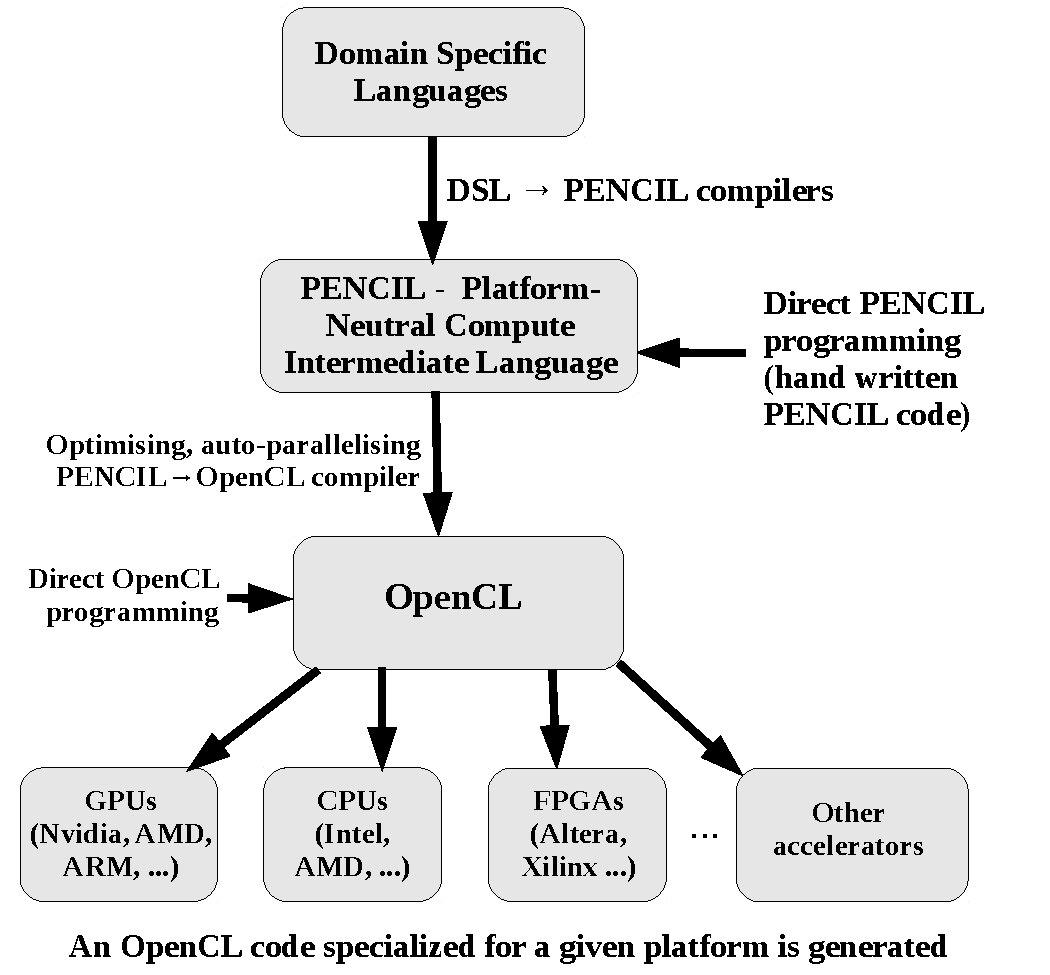
\includegraphics[scale=0.65]{./figures/CARPHighLevelOverview.pdf}
 \caption{High level overview of how \pencil should be used}
 \label{fig-pencil-high-level-picture}
} 
\end{figure}

Figure \ref{fig-pencil-high-level-picture} shows a high level
overview of how \pencil should be used.
First, a program written in a domain
specific language is translated into \pencil.  Domain specific
optimizations are applied during this translation.  Domain specific
information is also added, during this step, through specific \pencil language
constructs.  Second, the generated \pencil code is combined with
hand-written \pencil code that implements specific library
functions.  \pencil is used here as a standalone language.  The
combination of the two pieces of code is then optimized and
parallelized (using a polyhedral framework).  Finally, highly
specialized OpenCL code is generated.

In this document, we only deal with the source-level \pencil syntax.
We are putting a strong emphasis on the definition of constraints and
extensions that may be easily
lowered to compiler intermediate representations using attributes and built-in
functions.

\paragraph*{Notation}

Throughout this document, the notation \lstinline![OPT[CLAUSE]OPT]! indicates
that \lstinline!CLAUSE! is optional.

Section~\ref{pencil-c99-subset} presents the subset of C99 that
defines the core of \pencil, while Section~\ref{pencil-extension-short}
presents the extensions that are a part of \pencil.

\section{\pencil Definition as a Subset of C99}
\label{pencil-c99-subset}
The language syntax is defined in \figref{pencil-syntax} as an EBNF (Extended
Backus-Naur Form) grammar~\cite{wirth1996EBNF}.
The reserved words are in bold.
\pencil-specific types, built-in functions and macros are declared in
the \texttt{pencil.h}~\footnote{https://github.com/carpproject/}
header file.

\newcommand{\pgrammar}[1]{\text{\sf\textless#1\textgreater}}
\newcommand{\pkeyword}[1]{\mathbf{#1}}
\newcommand{\plexer}[1]{\text{\bf'#1'}}

\begin{figure}
\[
\begin{array}{lcl}
  \pgrammar{pencil} & \gets &  \pgrammar{top level definition}*\\
  \pgrammar{top level definition} & \gets & \pgrammar{function}
                                          | \pgrammar{type definition}
                                          | \pgrammar{global constant}\\

  \pgrammar{global constant} & \gets & \pgrammar{variable declaration}
                                       \plexer{=}
                                       \pgrammar{init expression} \plexer{;}\\

  \pgrammar{type definition} & \gets & (\pgrammar{typedef}
                                     | \pgrammar{struct definition}) \plexer{;}\\

  \pgrammar{typedef} & \gets & \pkeyword{typedef} \pgrammar{base type} \pgrammar{name} \pgrammar{array suffix}*\\

  \pgrammar{struct definition} & \gets & \pkeyword{struct} \pgrammar{name}
                                         \plexer{\{}
                                           (\pgrammar{variable declaration} \plexer{;})*
                                         \plexer{\}}\\

  \pgrammar{array suffix} & \gets & \plexer{[}
                                     (\pgrammar{array attribute}*) \pgrammar{expression}
                                    \plexer{]}\\

  \pgrammar{array attribute} & \gets & \pkeyword{const} | \pkeyword{restrict} | \pkeyword{static}\\

  \pgrammar{pointer} & \gets &  \plexer{*}\\

  \pgrammar{declarator} & \gets & (\pgrammar{pointer}*) \pgrammar{direct declarator}\\

  \pgrammar{direct declarator} & \gets & \pgrammar{name} (\pgrammar{array suffix}*)
                                       | \plexer{(} \pgrammar{declarator} \plexer{)} \pgrammar{array suffix}*\\

  \pgrammar{base type} & \gets & \pgrammar{scalar type fragment}+
                               | \pgrammar{type attribute}* \pkeyword{struct}? \pgrammar{name}\\


  \pgrammar{scalar type fragment} & \gets & \pgrammar{type specifier} | \pgrammar{type attribute} \\

  \pgrammar{type attribute} & \gets & \pkeyword{const} \\

  \pgrammar{type specifier} & \gets & \pkeyword{bool}
                                    | \pkeyword{\_Bool}
                                    | \pkeyword{char}
                                    | \pkeyword{short}
                                    | \pkeyword{int}
                                    | \pkeyword{long}
                                    | \pkeyword{float}
                                    | \pkeyword{half}
                                    | \pkeyword{double}
                                    | \pkeyword{signed}
                                    | \pkeyword{unsigned}
  \\

  \pgrammar{variable declaration} & \gets & \pgrammar{base type} \pgrammar{declarator}
  \\

  \pgrammar{init expression} & \gets & \pgrammar{expression} | \pgrammar{array init expression} \\

  \pgrammar{array init expression} & \gets & \plexer{[}\plexer{]}
                                           |\pgrammar{constant}\\
  & &                                      | \plexer{[} \pgrammar{array init expression}
                                                        (\plexer{,} \pgrammar{array init expression})*
                                             \plexer{]}
  \\
  \pgrammar{function} & \gets & \pkeyword{static}? \pgrammar{function type} \\
                                & & \pgrammar{name}
                                \plexer{(} \pgrammar{function args} \plexer{)} \pgrammar{attribute}*\\
                                & & \pgrammar{function body}
  \\
  \pgrammar{function type} & \gets & \pgrammar{base type} | \pkeyword{void} \\

  \pgrammar{function body} & \gets & \pgrammar{block} | \plexer{;}\\

  \pgrammar{attribute} & \gets & \pkeyword{\_\_attribute\_\_} \plexer{(}\plexer{(} \pgrammar{attr} \plexer{)}\plexer{)}\\

  \pgrammar{attr} & \gets & \pkeyword{const} 
                          | \pkeyword{pencil} 
                          |\pkeyword{pencil\_access} \plexer{(} \pgrammar{name} \plexer{)}
\\

  \pgrammar{function args} & \gets & | \pgrammar{variable declaration} (\plexer{,} \pgrammar{variable declaration})*\\

  \pgrammar{block} & \gets & \plexer{\{} \pgrammar{statement} * \plexer{\}}\\

  \pgrammar{statement} & \gets & \pgrammar{assignment} \plexer{;}
                               | \pgrammar{for}
                               | \pgrammar{while}
                               | \pgrammar{if}
                               | \pgrammar{block}
                               | \pgrammar{return}\\ & &
                               | \pgrammar{block variable declaration}
                               | \pgrammar{call statement}\\ & &
                               | \pkeyword{break} \plexer{;}
                               | \pkeyword{continue} \plexer{;}
  \\

  \pgrammar{assignment} & \gets & \pgrammar{lvalue}\\&& (\plexer{=}
                                                        | \plexer{+=}
                                                        | \plexer{-=}
                                                        | \plexer{\%=}
                                                        | \plexer{*=}
                                                        | \plexer{/=}
                                                        | \plexer{\textasciicircum=}
                                                        | \plexer{\&=}
                                                        | \plexer{$|$=}
                                                        | \plexer{\textgreater\textgreater=}
                                                        | \plexer{\textless\textless=})\\&&
                                                         \pgrammar{expression}\\ & &
                                                      | \pgrammar{lvalue} \plexer{++}
                                                      | \pgrammar{lvalue} \plexer{{-}{-}}\\&&
                                  |\plexer{++} \pgrammar{lvalue}
                                  |\plexer{{-}{-}} \pgrammar{lvalue}\\

  \pgrammar{while} & \gets & \pkeyword{while} \plexer{(} \pgrammar{expression} \plexer{)} \pgrammar{block}\\

  \pgrammar{if} & \gets & \pkeyword{if} \plexer{(} \pgrammar{expression} \plexer{)} \pgrammar{block}
  (\pkeyword{else} \pgrammar{block})?\\

  \pgrammar{return} & \gets & \pkeyword{return} \pgrammar{expression}? \plexer{;}\\

  \pgrammar{block variable declaration} & \gets &
  \pgrammar{variable declaration} (\plexer{=} \pgrammar{init expression})? \plexer{;}\\

  \pgrammar{call statement} & \gets & \pgrammar{call expression} \plexer{;}\\

\end{array}
\]
  \caption {\pencil{} syntax as an EBNF.}
  \label{fig:pencil-syntax}
\end{figure}

\begin{figure}
  \ContinuedFloat
\[
\begin{array}{lcl}
  \pgrammar{for directive} & \gets & \plexer{\#} \pkeyword{pragma} ~ \pkeyword{pencil} (\pkeyword{ivdep} | \pgrammar{independent})\\

  \pgrammar{independent} & \gets & \pkeyword{independent} (\pgrammar{reduction})*\\

  \pgrammar{name list} & \gets & \pgrammar{name} (\plexer{,} \pgrammar{name})*\\
  \pgrammar{reduction} & \gets & \pkeyword{reduction} \plexer{(} (\plexer{+}|\plexer{-}|\plexer{*}|\pkeyword{min}|\pkeyword{max}) \plexer{:} \pgrammar{name list}\plexer{)}\\

  \pgrammar{for step} & \gets & \plexer{++} \pgrammar{name}
  | \plexer{{-}{-}} \pgrammar{name}
  | \pgrammar{name} \plexer{++}
  | \pgrammar{name} \plexer{{-}{-}}\\&&
  | \pgrammar{name} \plexer{{+}=} \pgrammar{constant}
  | \pgrammar{name} \plexer{{-}=} \pgrammar{constant}\\

  \pgrammar{for} & \gets & \pgrammar{for directive}*\\&& \pkeyword{for} \plexer{(}
  \pgrammar{base type}? \pgrammar{name} \plexer{=} \pgrammar{expression} \plexer{;}\\&&
    ~ ~ ~ ~\pgrammar{name} (\text{\textgreater}|\text{\textless}|\text{\textgreater=}|\text{\textless=}) \pgrammar{expression}\plexer{;}\\&&
    ~ ~ ~ ~\pgrammar{for step} \plexer{)}\\&&\pgrammar{block}\\

  \pgrammar{expression} & \gets & \pgrammar{ternary expression}\\

  \pgrammar{ternary expression} & \gets & \pgrammar{LOR expression}
  (\plexer{?} \pgrammar{expression} \plexer{:} \pgrammar{ternary expression})?\\

  \pgrammar{LOR expression} & \gets & \pgrammar{LAND expression} (\plexer{$||$} \pgrammar{LAND expression})*\\

  \pgrammar{LAND expression} & \gets & \pgrammar{BitOR expression} (\plexer{\&\&} \pgrammar{BitOR expression})*\\

  \pgrammar{BitOR expression} & \gets & \pgrammar{BitXOR expression} (\plexer{$|$} \pgrammar{BitXOR expression})*\\

  \pgrammar{BitXOR expression} & \gets & \pgrammar{BitAND expression} (\plexer{\textasciicircum} \pgrammar{BitAND expression})*\\

  \pgrammar{BitAND expression} & \gets & \pgrammar{EQ expression} (\plexer{\&} \pgrammar{EQ expression})*\\

  \pgrammar{EQ expression} & \gets & \pgrammar{CMP expression} ((\plexer{=}|\plexer{!=}) \pgrammar{CMP expression})*\\

  \pgrammar{CMP expression} & \gets & \pgrammar{shift expression} (
               (\plexer{\textgreater}
               |\plexer{\textless}
               |\plexer{\textgreater=}
               |\plexer{\textless=})
               \pgrammar{shift expression})*\\

  \pgrammar{shift expression} & \gets & \pgrammar{plus expression} (
       (\plexer{\textless\textless}|\plexer{\textgreater\textgreater}) \pgrammar{plus expression})*\\

  \pgrammar{plus expression} & \gets & \pgrammar{mult expression} ((\plexer{+}|\plexer{-}) \pgrammar{mult expression})*\\

  \pgrammar{mult expression} & \gets & \pgrammar{cast expression} ((\plexer{*}|\plexer{/}|\plexer{\%}) \pgrammar{cast expression})*\\

  \pgrammar{cast expression} & \gets & (\plexer{(} \pgrammar{scalar type fragment}+ \plexer{)})* \pgrammar{unary expression}\\

  \pgrammar{unary expression} & \gets & \plexer{~} \pgrammar{cast expression}
                              | \plexer{-} \pgrammar{cast expression}\\&&
                              | \plexer{+} \pgrammar{cast expression}
                              | \plexer{!} \pgrammar{cast expression}\\&&
                              | \pgrammar{sizeof expression}
                              | \pgrammar{postfix expression}\\

  \pgrammar{lvalue} & \gets & \pgrammar{subscription}\\

  \pgrammar{postfix expression} & \gets & \pgrammar{call expression} | \pgrammar{subscription}\\

  \pgrammar{call expression} & \gets & \pgrammar{name} \plexer{(}
  (\pgrammar{expression} (\plexer{,} \pgrammar{expression})*)?
  \plexer{)}\\

  \pgrammar{subscription} & \gets & \pgrammar{term} (\plexer{[} \pgrammar{expression} \plexer{]} |
                                                     \plexer{.} \pgrammar{name})*\\

  \pgrammar{term} & \gets & \pgrammar{name} | \pgrammar{constant} | \plexer{(} \pgrammar{expression} \plexer{)}\\

  \pgrammar{constant} & \gets & \pgrammar{HEX humber} | \pgrammar{DEC number} | \pgrammar{OCT number}\\&&
  | \pgrammar{Floating point number}\\
\end{array}
\]
  \caption {\pencil{} syntax as an EBNF continued.}
\end{figure}


\subsection{Program Scope}
The following \C global definitions are allowed inside a \pencil program:
\begin{itemize}
  \item Type definition;
  \item Function declaration;
  \item Function definition;
  \item Global constants definition (unlike \C, only constant global variables
        are allowed in \pencil)
\end{itemize}

\subsection{Types}
Types are defined in \pencil in the same way as in \C but
only the following \C types are allowed inside a \pencil program.
\begin{itemize}
  \item Scalar types (same as in \C)
      \footnote{half float type (\lstinline!half!) in \pencil is an optional
      type, \pencil compilers are not required to support it.}
  \item Array types
  \begin{itemize}
    \item Arrays must be declared using the C99
      variable-length array syntax~\cite{c99}, array function arguments
      must be declared using the \lstinline!restrict! and
      the \lstinline!const! type qualifiers, and the \lstinline!static! keyword
      described in sections~\ref{sec:restrict},~\ref{sec:const}
      and~\ref{sec:static}.
    \item Array accesses should not be linearized, as this tends to
      obfuscate affine subscript expressions.  Multidimensional C99 arrays
      should be used instead even for function arguments (variable-length arrays
      C99 syntax).
    \item In order to have a precise dependence analysis, it is recommended
      to use quasi-affine array subscripts (Section~\ref{sec:quasi-affine})
      whenever this is possible.
  \end{itemize}
  \item Structural types (same as in \C)
  \item Pointers types
  \begin{itemize}
    \item Pointer declaration and definition are allowed in
      \pencil to allow the use of non-\pencil libraries (since the header files
      of non-\pencil libraries may contain pointer declarations).
    \item Pointer manipulation (including array arithmetic and reading or
      writing to a pointer) is not allowed.  There is one exception to this
      restriction, reading an array reference is allowed when the reference is
      passed in a function call (\eg \lstinline!mat_add(C, A, B)!).
    \item Pointer dereferencing is not allowed.  The only exception to
      this is accessing arrays using array subscripts
      (\eg \lstinline!A[i][j]!).
    The restricted use of pointers is important for moving data between
    different address spaces of hardware accelerators, as it essentially
    eliminates aliasing problems.
  \end{itemize}    
\end{itemize}
Unlike \C, unions and bitfields are not supported in \pencil.

\subsection{Functions}
Function definition and declaration in \pencil are identical to function
definition and declaration in \C.
Function overloading and recursion are not allowed (note that OpenCL does
not support recursion anyway).
\pencil provides additional
function annotations covered later in the document. \pencil functions can
be called from \C programs.

\subsection{Statements}
The following \C statements are allowed inside a \pencil function definition:
\begin{itemize}
  \item Assignment;
  \item For loop;
  \item While loop;
  \item If statement;
  \item Compound statement;
  \item Break statement;
  \item Continue statement;
  \item Return statement (should be used only at the end of a function);
  \item Call statement.
\end{itemize}
Unlike \C, \lstinline!goto! Statements are not allowed in \pencil.
See detailed descriptions below.

\subsubsection{Assignment}
\label{sec:assignments}
The following \C assignment statements are supported:
\begin{itemize}
  \item Basic assignment: \lstinline!=!
  \item Compound assignment: \lstinline{+=, -=, *=, /=, %=, |=, &=, ^=, <<=, >>=}
\end{itemize}

Unlike in \C, the \pencil assignment does not return any value (\ie
it is a statement, not an operator).
The goal is mainly to simplify the development of \pencil tool chains.
For example, the following case is illegal in \pencil:
\begin{lstlisting}[language=pencil]
  int i = 2; //OK.
  int j = i += 2; //OK in C99, illegal in PENCIL.
\end{lstlisting}

As a special case \lstinline!i += 1! can be written as \lstinline!i++!
and \lstinline!i -= 1! can be written as \lstinline!i--!, but as mentioned
above these constructions are statements without any return value:

\begin{lstlisting}[language=pencil]
  int j = i++; //Legal in C99, illegal in PENCIL.
  i++; // Legal in C99 and in PENCIL.
\end{lstlisting}

\subsubsection{For Loop}

A \pencil for loop must have a single iterator, an invariant start
value, an invariant stop value and a literal constant increment (step).
Invariant in this context means that the value does not change within
the loop body.

\begin{lstlisting}[language=pencil]
  for (type iter = init; iter [<|<=|>|>=] bound; iter[+|-]=step)
  {
    //Body
  }
\end{lstlisting}
The iteration variable is not visible outside the loop and cannot be modified
inside the loop body.

By precisely specifying the loop format, we avoid the need for
a sophisticated induction variable analysis.
Such an analysis is not only complex to implement, but more
importantly results in compiler analyses to succeed or fail under
conditions unpredictable to the user.

In order to have a precise dependence analysis, it is recommended
to use quasi-affine loop bounds (Section~\ref{sec:quasi-affine}).

A for loop can be annotated with additional directives
(see Section~\ref{sec:for-directives}).
\subsubsection{While Loop}
The same as in \C.
\subsubsection{If Statement}
The same as in \C.
In order to have a precise dependence analysis, it is recommended
to use quasi-affine conditional expressions (Section~\ref{sec:quasi-affine})
whenever this is possible.
\subsubsection{Break Statement}
The same as in \C.
\subsubsection{Continue Statement}
The same as in \C.
\subsubsection{Return Statement}
The same as in \C except that it can be used only at the end of a function
(\ie as the last statement in a function body).
\subsubsection{Call Statement}
The same as in \C except that
\begin{itemize}
 \item Calling a non-\pencil function from \pencil
 is allowed only if its summary functions is provided.
 \item Recursive function calls are not allowed.
\end{itemize}

\subsection{Expressions}
\pencil supports a strict subset of \C expressions:
\begin{itemize}
  \item Arithmetical operations: \lstinline!+,-,*,/,%!
  \item Logical operations: \lstinline{||,&&,!}
  \item Bit operations: \lstinline{|,&,~,^,>>,<<}
  \item Comparison operations: \lstinline{>,>=,<,<=,==,!=}
  \item Array and member operators: \lstinline{[],.}
  \item Ternary conditional: \lstinline!cond?op1:op2!
  \item Size-of: \lstinline!sizeof(arg)!
  \item Scalar conversion: \lstinline!(type)arg!
  \item \pencil function call: \lstinline!func(arg1,..,argN)!
  \item C function call (when the summary function is provided).
\end{itemize}

Unlike C, where any expression can be used as a statement, in
order to simplify the development of \pencil tool chains, \pencil
restricts the set of expressions that can be used as statements
to the following list:
\begin{itemize}
    \item Function calls:
        \begin{lstlisting}
            foo(bar(1),2);
        \end{lstlisting}
    \item Compound assignments
        \begin{lstlisting}
            i += 2;
        \end{lstlisting}
    \item pre-/post- increment/decrement operations.
        \begin{lstlisting}
            i++;
        \end{lstlisting}
\end{itemize}


\subsection{Quasi-affine Expressions}
\label{sec:quasi-affine}

A quasi-affine expression is any expression over integer values and
integer variables involving only the operators \lstinline{+},
\lstinline{-} (both unary and binary), \lstinline{*}, \lstinline{/},
\lstinline
operators is required to be a (positive) integer literal, while at
least one of the arguments of the \lstinline{*} operator is
required to be piece-wise constant expression. An example of a
quasi-affine expression is: $a*i+b*j+c$, where $a$ and $b$ are
constants and $c$ is either a constant or a loop parameter.

It is recommended to use quasi-affine expressions for
array subscript, loop bounds, conditional expressions,
and to specify memory access information (described in
section \ref{sec:mem-acces-info}).

\begin{lstlisting}[language=pencil]
for (int i=1; i<n; i++) {
  A[10*i+20] = 0;	// Quasi-affine
  A[i*n] = 0;		// Not quasi-affine
  B[i*i] = 0;		// Not quasi-affine
  C[t[i]] = 0;		// The subscript of C[] is not quasi-affine
  D[foo(i)] = 0;	// Not quasi-affine
}
\end{lstlisting}

In presence of non quasi-affine subscripts, it is highly recommended
to use the \lstinline!independent! or \lstinline!ivdep! directives to
enable parallelization and loop optimizations, or to hide these
accesses in (possibly \lstinline!inline!) functions annotated with
memory access information.

\section{\pencil Extensions to C99}
\label{pencil-extension-short}

This section provides a list of \pencil extensions, the detailed
description of these extensions is provided
in~\ref{sec:Annotations-and-directives}

\subsection*{Directives}
\label{sec:for-directives}

\begin{itemize}
\item \lstinline!#pragma pencil independent [OPT[reduction(operator: scalar_1, $\ldots$, scalar_n)*]OPT]!
\item \lstinline!#pragma pencil ivdep!
\item \lstinline!#pragma pencil access!
\item \lstinline!#pragma pencil region!
\end{itemize}

\subsection*{Keywords and Type Qualifiers for Array Arguments}

\begin{description}
  \item \lstinline!const!
  \item \lstinline!restrict!
  \item \lstinline!static!
\end{description}

\subsection*{Type Attributes}

\begin{description}
  \item \lstinline!__attribute__((pencil_heap))!
\end{description}

\subsection*{Function Attributes}

\begin{description}
  \item \lstinline!__attribute__((pencil_access()))!
  \item \lstinline!__attribute__((const))!
  \item \lstinline!__attribute__((pencil))!
\end{description}

\subsection*{Built-in Functions}

\begin{itemize}
\item \lstinline!__pencil_kill!;
\item \lstinline!__pencil_use!;
\item \lstinline!__pencil_def!;
\item \lstinline!__pencil_maybe!;
\item \lstinline!__pencil_assume!;
\item \lstinline!__pencil_assert!.
\end{itemize}

\chapter{Detailed Description of the Extensions to C99}
\label{sec:Annotations-and-directives}

\section{Keywords, Type Qualifiers and Type Attributes for Array Declaration}
\label{sec:array-type-qualifiers-section}

\subsection{\lstinline!static! Keyword}
\label{sec:static}

\begin{description}
\item [Usage] Used when declaring an array argument of a \pencil function.
\item [Description] The \lstinline!static! keyword in \pencil
has the same semantics as the \lstinline!static! keyword in C99.
All array arguments of a \pencil function
must be declared using the \lstinline!static! keyword.
The use of this type qualifier is
important to implement array expansion or data transfers when
subscripts are not affine.%
\footnote{An array expansion maps an array to a larger array, typically
by adding extra dimensions.  The mapping may depend on the statement
instance and can be used to remove some memory reuse.}
\end{description}

\subsection{\lstinline!const! Type Qualifier}
\label{sec:const}

\begin{description}
\item [Usage] Used when declaring an array argument of a \pencil function.
\item [Description] The \lstinline!const! type qualifier in \pencil
has the same semantics as the \lstinline!const! type qualifier in C99.
All array arguments of a \pencil function
must be declared using the \lstinline!const! type qualifier.
It is used to make sure that array arguments behave as closely as possible to
array variables, and to forbid that array arguments (the base
pointer, not individual elements) occur at the left-hand side of an
expression.  This rule eliminates the risk of inducing array aliasing
through the assignment of an arbitrary base address to an array
argument.
\end{description}

All array arguments in a \pencil function must be
qualified by \lstinline!static const!.

\subsection*{Examples}

Here is a correct \pencil function declaration and call.

\begin{lstlisting}[language=pencil]
/* PENCIL code.  */
void foo(int n, float a[static const n]);

void bar()
{
  int n = 42;
  float pa[n];

  foo(n, pa);
}

/* C code.  */
void baz ()
{
  /* Note: this is a C code that calls a PENCIL function,
  it is not a PENCIL code.  */

  int n = 42;
  float *buf = malloc (sizeof (*buf) * n);
  foo (n, buf);
}
\end{lstlisting}

\subsection{\lstinline!restrict! Type Qualifier}
\label{sec:restrict}

% A discussion about whether the restrict keyword should be kept in PENCIL
% or not.  The advantage of keeping restrict is to be compatible with the
% C programming style where safety is not the default, and safety (restrict)
% is indicated using a keyword.

\begin{description}

\item[Usage] Used when declaring an array argument of a \pencil function.

\item[Description] This qualifier has the same syntax and semantics
  as in C99.
  It allows the compiler to know if array
  arguments are aliased, which enables the compiler to
  perform more precise dependence analysis.
  
  Usage of this qualifier is \emph{not} mandatory.
  Making the use of \lstinline!restrict! mandatory would require
  upstream versioning of functions which increases the effort
  for writing and generating \pencil code.
  For modularity and reuse, it is more interesting to let \pencil
  front-end(s) handle the versioning and specialization themselves.
  E.g., from a generic \lstinline!memcpy! function, create two versions
  for the aliased and unaliased cases.

\item[Example]~
  \begin{lstlisting}[language=pencil]
// a and b may be the same array (or partially overlap)
// in foo_alias
void foo_alias(float a[const static 42],
                 float b[const static 42]);

// a and b are restricted arrays (analogous to restricted
// pointers in C99)
void foo_restricted(float a[static const restrict 42],
                     float b[static const restrict 42]);
  \end{lstlisting}
\end{description}

\todo{Perhaps we should make an exception for
  dynamic memory allocation.  In that case, the allocated address
  should be held in a pointer-to-array type, not a
  pointer-to-scalar/struct type in order to preserve size information.
  An old revision (svn r552) of this document has an example, but the
  details are still in the works.}

\subsection{\lstinline!pencil\_heap! Type Attribute}
\label{sec:heap-attribute}
 
\begin{description}
\item[Usage] The \lstinline!pencil_heap! attribute
  (\lstinline!__attribute__((pencil_heap))!) can be used when declaring
  an array using the C99 VLA syntax within a \pencil code
  \footnote{The C99 VLA syntax is the only syntax that can be used
    to declare arrays in \pencil.}.
  It should not be used for array arguments.
  
\item[Description] This attribute forces the compiler to allocate
  heap memory for the array being declared.

\item[Abbreviation] The \lstinline!HEAP! macro abbreviates
  \lstinline!__attribute__((pencil_heap))!.
  
\item[Example]~
  \begin{lstlisting}[language=pencil]
    // array is allocated on the heap
    int array[10000] HEAP;
  \end{lstlisting}
\end{description}

\section{Function Attributes}

A \pencil compiler is not supposed to perform interprocedural analysis or to
apply transformations across function definitions.
%TODO: explain why
A description of the memory accesses of a function called from a \pencil
region must be provided (Section~\ref{sec:mem-acces-info-for-functions}),
unless the function is a \pencil function
or is annotated with \lstinline!const! (see Section~\ref{sec:const-attribute}).

\subsection{\lstinline!const! Function Attribute}
\label{sec:const-attribute}

\begin{description}
\item[Description] The \lstinline!const! attribute of GCC is allowed in
  \pencil for compatibility with existing \lstinline!const!-annotated
  library functions (e.g., \lstinline!cos!, \lstinline!sin!, \lstinline!min!,
  \lstinline!max!, etc.).

\item[Abbreviation] The \lstinline!CONST! macro abbreviates
  \lstinline!__attribute__((const))!.
\end{description}
  
\section{Description of Memory Accesses}
\label{sec:mem-acces-info}
We first show the annotation used to represent memory access information
of functions, then we show the equivalent inline annotation that can be used
for statements and blocks.

\subsection{Description of Memory Accesses for Functions}
\label{sec:mem-acces-info-for-functions}

% Note: Semantics (albert):
% - it is plain C code with some restrictions that the only non-scalar
%   accesses are USE/DEF with;
% - the semantics of USE/DEF is nop; as a corollary, a summary function has
%   no side effect, it is pure;
% - calls to other summaries are allowed.

\begin{description}
  \item [Usage] The name of a summary function is indicated through
  the \lstinline!pencil_access! function attribute.

  \item [Description] The goal is to describe how the arguments of a given
  function are accessed.
  For each array (or scalar) passed to the function,
  a description of the memory accesses to that array is provided.
  This information is important for performing a precise dependence
  analysis.
  It can be provided through a summary function.
  
  Summary functions are used to:
    \begin{itemize}
     \item Describe the memory accesses of library functions
     called from \pencil code --- as library functions cannot be analyzed at
     compile time.
     If the memory access of a function is not provided, a \pencil
     compiler assumes that every argument of the function is fully accessed
     for read and write.
     
     \item Describe the memory accesses of non-\pencil
     functions called from \pencil code --- as they are difficult
     to analyze.

     \item Describe the memory accesses of \pencil functions with complex
     memory access patterns.
     Although the compiler can perform memory access analysis automatically,
     it may perform a conservative analysis and may over-approximate the
     actual access patterns.  In this case, memory access information should
     be specified.
    \end{itemize}

  The use of summary functions in these cases enables more
  precise static analysis.

  To indicate the summary function of a function \lstinline!foo!,
  one should use the attribute \lstinline!pencil_access(summary)! where
  \lstinline!summary! is the name of the summary function  that describes
  the memory accesses in \lstinline!foo!.
  
  Example:
  \begin{lstlisting}[language=pencil]
    /* This is the summary function of foo().  */
    void foo_summary(int N, int A[static const restrict N])
    {
      /* The contents of summary functions will be presented
      later in this section.  */
    }

    void foo(int N, int A[static const restrict N])
      __attribute__((pencil_access(foo_summary)))
      {
        for (int i = 0; i < N; i ++)
        {
          A[i] = A[i] + 1;
        }
      }
  \end{lstlisting}
  
  The summary function has the same arguments as the
  qualified function.  Each array that is passed as an argument to the
  function must be described.
  However, it is not meant to be executed: it is only
  useful for the dependence analyzer.
  
  The semantics of
  memory access information are equivalent to the semantics
  of interprocedural function summaries.  A simple way to integrate
  it in an existing intraprocedural framework is to inline all
  summaries.

  Note that summaries should always appear in source form,
  preferably in headers, and that the summary function itself
  should be \pencil compliant so that \pencil tools can
  analyze it.
  
  A summary function does not describe the dependences between the
  different statements of the function.  It is intended to describe
  the dependences between the function call, seen as one statement,
  and the rest of the call site code.

  The polymorphic built-in functions \lstinline!__pencil_use!
  and \lstinline!__pencil_def! must be used in summary
  functions to mark memory access information (and to protect them
  from aggressive, \pencil-agnostic upstream passes). The
  polymorphic argument may be a scalar,
  dereferenced pointer argument, or array element. It may also be a
  complete array when the dimension and size of the array are
  statically known (use the \lstinline!static! keyword for
  arguments): e.g., \lstinline!__pencil_use(A)! marks the use of the
  complete array A, alleviating the need to list every
  element.

  In this document we use the following abbreviating macros:
  \lstinline!USE()! and \lstinline!DEF()!
  \begin{itemize}
   \item \lstinline!USE()! is used to abbreviate \lstinline!__pencil_use!.
         It annotates read accesses.
   \item \lstinline!DEF()! is used to is used to abbreviate \lstinline!__pencil_def!.
         It annotates (must-)write accesses.
  \end{itemize}

  To express may-write accesses, the boolean built-in
  \lstinline!__pencil_maybe! should be used to guard these accesses
  in an \lstinline!if (__pencil_maybe())!  conditional. We use the
  \lstinline!MAYBE! macro as an abbreviation. The
  built-in may be combined with more (affine) conditions to refine
  the static may-execute information. One may also consider
  \lstinline!MAY_DEF(v)! as a short-cut for
  \lstinline!if (__pencil_maybe()) __pencil_def(v))!.

  A summary function can contain calls to other functions, indicating,
  that corresponding calls are present on the original function:

  \begin{lstlisting}[language=pencil]
    void foo(int N, int A[static const restrict N]);

    void bar_summary(int N, int A[static const restrict N])
    {
      foo(N, A);
      USE(A);
      DEF(A);
    }

    void bar(int N, int A[static const restrict N])
      __attribute__((pencil_access(bar_summary)))
      {
        foo(N, A);
        for (int i = 0; i < N; i ++)
        {
          A[i]++;
        }
      }
  \end{lstlisting}

  \item[Abbreviation] The attribute \lstinline!pencil_access! is
  abbreviated with the \lstinline!ACCESS! macro.
  
  The summary function does not need to preserve information about
  the dependences between the different statements of the function.
  If an argument is read (resp. written) multiple times, it is enough
  to indicate this only once in the summary function.

  The main criteria for choosing a given formalism instead of another
  formalism to express the memory accesses of a function are:
  \begin{itemize}
   \item the expressivness of the formalism;
   \item the ease of expressing memory accesses in the formalism;
   \item the ability to use existing compilation frameworks to parse
         and analyze the formalism.
  \end{itemize}

  Summary functions were chosen over other formalisms because they are based
  on the C syntax and thus can be parsed and analyzed easily using existing C
  compiler APIs.
  Moreover, summary functions are expressive and allow fine grain
  specification of memory accesses.
  And more importantly, summary functions are easy to understand unlike other
  formalisms like lambda expressions (not all C programers are familiar with
  the concept of lambda expressions).
  
%   \item[Example 1]~
%   The following example shows a function (\lstinline!bar!)
%   and its summary (\lstinline!bar_summary!).
%    \begin{lstlisting}[language=pencil]
% void bar_summary(int n, int A[static const restrict n],
%                        int B[static const restrict n])
% {
%   for (int i=0; i<n; i++) {
%     USE(B[i]);
%     DEF(A[i]);
%     if (MAYBE)
%       DEF(B[i]);
%   }
% }
% 
% /* Or the equivalent, shorter version. */
% void bar_summary(int n, int A[restrict n],
%                        int B[restrict n])
% {
%   USE(B);
%   DEF(A);
%   MAY_DEF(B);
% }
% 
% void bar(int n, int A[static const restrict n],
%             int B[static const restrict n])
%             ACCESS(bar_summary(n,A,B))
% {
%   int i;
% 
%   for (i=0; i<n; i++) {
%     A[i] = B[i];
%     A[i] = A[i] + 1;
%     B[n * drand48()] = 42;
%   }
% }
%   \end{lstlisting}
% 
%   For each function argument written or read by the function, the
%   summary should contain a code that describes that access.  In the
%   example, the loop in \lstinline!bar_summary! is used to express a read
%   access on \lstinline!B[i]!, a write access on \lstinline!A[i]! and a
%   potential write access on \lstinline!B[i]! for \lstinline!i! going from
%   $0$ to $n-1$.

  
\item[Example 1]~
  \begin{lstlisting}[language=pencil]
  __attribute__((pencil_access(summary_fft32)))
  void fft32(int i, int j, int n,
              float in[pencil_attributes n][n][n]);

  int ABF(int n, float in[pencil_attributes n][n][n])
  {
    // ...
    for (int i = 0; i < n; i++)
    {
      // ...
      for (int j = 0; j < n; j++)
        fft32(i, j, n, in);
    }
    // ...
  }

  void summary_fft32(int i, int j, int n,
              float in[pencil_attributes n][n][n]);
  {
    for (int k=0; k<32; k++)
      __pencil_use(in[i][j][k]);
    for (int k=0; k<32; k++)
      __pencil_def(in[i][j][k]);
  }
  \end{lstlisting}
  
  This example shows a loop nest extracted from
  \emph{ABF} (Adaptive Beamformer), a signal processing kernel used in radar
  systems.
  The code calls the function \lstinline!fft32! (Fast Fourier Transform)
  which only reads and modifies (in place) 32 elements of its input
  array \lstinline!in!, it does not modify the whole input array.
  Such a function is not analyzed by the \pencil compiler as it is not a \pencil
  function.
  Without a summary function, the compiler assumes conservatively that the whole
  array passed to \lstinline!fft32! is accessed for read and for write.
  Such a conservative assumption prevents the parallelization of the code.
  The use of a summary function in this case indicates to the compiler that
  each iteration of the loop nest reads and writes to a 32 elements
  of the input array.
  This information allows the compiler to parallelize and optimize the loop
  nest.

  
  \item[Example 2]~
  \begin{lstlisting}[language=pencil]
struct complex {
  int image;
  int real;
};

typedef struct complex Cplx;

void foo_summary(int n, int A[static const restrict n],
                       Cplx d[static const restrict n])
{
  for (int i=0; i<n; i++)
    USE(A[i]);

  /* Note that i starts from 10. */
  for (int i=10; i<n; i++)
    MAY_DEF(d[i].real);

  DEF(A[15]);
}

void foo(int n, int A[static const restrict n],
            Cplx d[static const restrict n])
            ACCESS(foo_summary(n,A,Cplx))
{
  int i, t;

  for (i=0; i<n; i++)
    printf("Value=%d", A[i]);

  for (i=0; i<n; i++)
  {
    if (A[i])
      printf("%d", i);

    t += A[i];
  }

  for (i=0; i<n; i++)
    if (A[i] && i>10)
      d[i].real = t;

  A[15] = 0;
}
  \end{lstlisting}

  In the previous example, the summary function
  \lstinline!foo_summary!  indicates that the function
  \lstinline!foo! reads the values of \lstinline!A[i]!  for $i$
  from $0$ to $n-1$ and writes to \lstinline!A[15]!.
  \lstinline!foo! may write to \lstinline!d[i].real! for $i$
  from $10$ to $n-1$. 
\end{description}

\subsection{Inline Description of Memory Accesses for Statement Blocks}
\label{sec:inline-mem-access-info}

%\todo{AC. This is a rough proposal, in response to Alexey and Anton's draft.}

To simplify the annotation of short code regions, it is also possible to
add a description of memory accesses to arbitrary statements/blocks of code.
The syntax is the same as above, but with summary code inlined
directly into the \lstinline!#pragma pencil access! directive.

\begin{lstlisting}[language=pencil]
//Data access specified for the whole loop.
#pragma pencil access \
  { for (int i=0; i<N; i++) {USE(A[i]); DEF(B[i]);} }
for (int i = 0; i < N; ++i)
{
   /* Alternatively, the same data information can be specified
      for a single iteration. */
   #pragma pencil access { USE(A[i]); DEF(B[i]); }
   {
     B[i] = A[i] * 2;
   }
}

/* Alternative, the same previous information can be provided
   with a summary function, and short array
   notation. */
void summary1(int i, int n, float A[static const restrict n],
              float B[static const restrict n])
{
  USE(A[i]);
  DEF(B[i]);
}

//Data access specified for the whole loop.
#pragma pencil access { USE(A); DEF(B); }
for (int i = 0; i < N; ++i)
{
   /* Alternatively, the same data information can be specified
      for a single iteration. */
   #pragma pencil access { summary1(i, N, A, B); }
   {
     B[i] = A[i] * 2;
   }
}
\end{lstlisting}

In the examples above for both cases memory access information has been
specified twice - on the loop level and on the iteration level, although it is
sufficient to specify it only once.

One technical problem is that it is currently impossible to translate
such directives into attributes attached to a statement/block. GNU C,
as implemented in GCC and Clang, does not support it, and neither does
GIMPLE or LLVM IR.

% It may be possible to apply some outlining
% automatically, but the impact is not yet well understood.

\section{Pragma Directives}

\pencil defines several directives inspired by OpenMP and OpenACC
and commonly found in advanced vectorizing compilers.

\subsection{\lstinline!pencil independent! Directive}

\begin{description}
\item [Usage] Used to annotate loops.
It has the following form:
\begin{lstlisting}[language=pencil]
#pragma pencil independent [OPT[reduction(op: scal_1, $\ldots$, scal_n)]OPT]*
\end{lstlisting}

\item [Description]
% It indicates that for a given execution of the marked loop, if two
% distinct iterations access the same memory element of a shared
% variable, then both accesses are read accesses A variable is
% considered shared if it is not declared inside the loop body.

The directive indicates that the desired result of the annotated
loop does not depend upon the execution order of data accesses
from different iterations.  The definition of data accesses
encompasses all memory accesses enclosed by the loop, either directly
or indirectly through calls to PENCIL or non-PENCIL functions. In
particular, data accesses from different iterations may be executed
simultaneously. The definition of desired result is algorithm- and
application-dependent.

The execution order of data accesses may be entirely defined by
the dependences of the PENCIL program, in which case the semantics of
the pragma is portable. Or some dependences may exist and nonetheless
ignored through the usage of the \lstinline!independent! directive,
in which case the correct execution order may have to be guaranteed
using specific synchronization constructs.
Reductions implemented as atomic regions in the generated code are one
typical example. Low-level atomics in C11 or OpenCL 2.0 are another one
(e.g., to give semantics to benign races).

Indeed, external non-PENCIL functions called from the annotated loops
may employ target-dependent constructs to protect the atomicity of
their data access sequences, or to refine their parallel semantics
regarding relaxed memory ordering, sound implementation of benign
races, etc. These functions must have well-formed summaries, capturing
the side effects of all their array arguments.  Such an approach is
currently necessary to allow benign races (when the same value is
written by multiple threads), to parallelize associative and commutative
operations, and more generally for any parallel algorithm tolerating
the unordered execution of intermediate steps.

The \lstinline!independent! directive is typically used to indicate
that the annotated loop does not carry any dependence.  It allows the
compiler to ignore all loop carried dependences of the annotated loop,
including those that may be introduced by the compiler due to
conservative assumptions (for example, if the code contains non affine
write accesses).
Note that no implicit privatization of scalars and arrays is assumed when
the \lstinline!independent! directive is used.  Instead, scalars and
arrays that are privatizable should be declared as local variables
within the scope of the annotated loop.
This may sound overly restrictive, but it ensures the portability of
PENCIL when targeting languages and architectures where races have
undefined semantics (C11, OpenCL 2.0).

The \lstinline!independent! directive has an effect only on the marked loop
and does not have an effect on any other loop in the loop nest.

\item [Note]~
The independent directive currently has informal semantics only. There
are plans for more formal versions, or for the complete deprecation of
the directive, in future revisions of PENCIL.

\item [Example 1]~

  The following example illustrates the usage of the directive in a
  typical context where the code executed in the loop body executes
  target-dependent, non-PENCIL code. E.g., code with atomic execution
  constraints that are currently not expressible in PENCIL.
  \begin{lstlisting}[language=pencil]
void inc_summary(float A[256], int c)
{
  if (MAYBE)
  {
    USE(A);
    DEF(A);
  }
}

void inc(float A[static const restrict 256],
            int c) ACCESS(inc_summary);

void foo(int N, float A[static const restrict N], int c)
{
  #pragma pencil independent
  for (int i=0; i<N; i++)
    inc(a, t[i]);
}  
  \end{lstlisting}

  With the following non-PENCIL C code implementing \lstinline!inc!,
  provided in a different file and compiled separately.
  \begin{lstlisting}[language=pencil]
void inc(float A[256], int c)
{
  atomic_inc(&A[c]);
}
  \end{lstlisting}

  Different iterations of the loop in \lstinline!foo! may write to the
  same array location (as the locations written depend on the values of
  \lstinline!t[i]!, which may not be unique).
  To parallelize the loop, the compiler
  needs to make sure that there is no loop-carried dependence, but
  proving this property is generally not possible at compile time.  Thus, the
  compiler must assume conservatively that there may be a dependence
  between different iterations and not parallelize the loop.
  If, for example, the \pencil programmer knows that all values of
  \lstinline!t[i]! are different, she
  should insert an \lstinline!independent! directive to indicate that different
  iterations of the loop are independent. This will allow the compiler to
  parallelize the loop, but also provide valuable
  information for other loop transformations.

\item [Example 2]~
  In the following example, the writes to \lstinline!t! induce loop carried
  dependences and thus the use of \lstinline!independent! is incorrect because
  there are at least two iterations that may write different values to
  \lstinline!t!.

  \begin{lstlisting}[language=pencil]
int t;
#pragma pencil independent
for (int i=0; i<N; i++) {
  t = foo(i);
  A[B[i]] = t;
}
  \end{lstlisting}  
  
  To be able to use \lstinline!independent! in the previous example, the
  scalar \lstinline!t! has to be declared in the loop body, this way each
  iteration will have its own copy of \lstinline!t! and thus the writes to
  \lstinline!t! by different iterations will not induce any loop carried
  dependence.  This is possible because \lstinline!t! is privatizable (\ie
  can be made private).
  The following example is correct.

  \begin{lstlisting}[language=pencil]
#pragma pencil independent
for (int i=0; i<N; i++) {
  int t = foo(i);
  A[B[i]] = t;
}
  \end{lstlisting}
   
  In general, all the variables declared inside the loop body (whether the loop
  is marked as independent or not) can be assumed to be free of loop-carried
  dependences (i.e., these variables do not induce any loop carried dependence).

\item [Example 3]~
  The following example shows a code fragment of a \pencil
  implementation of the breadth-first search algorithm.
  This algorithm computes the minimal distance from a given source node to
  each node of the input graph.
  The algorithm maintains a frontier and computes the next frontier by examining
  all unvisited nodes adjacent to the nodes of the current frontier.
  All nodes in a frontier have the same distance from the source node.

  The \lstinline|for| loop shown in the example can be
  parallelized since each node of the current frontier can be processed
  independently.
  This creates a possible race condition on the \lstinline|cost| and
  \lstinline|next_frontier| arrays.
  The race condition can be ignored, however, because each conflicting thread
  will write the same values to the arrays.
  By specifying the \lstinline|independent| pragma, the programmer guarantees
  that the race condition is benign, which enables a \pencil compiler to
  parallelize the loop.

  \begin{lstlisting}[language=pencil]
  /* Examine nodes adjacent to current frontier */
  #pragma pencil independent
  for (int i = 0; i < n_nodes; i++) {
    if (frontier[i] == 1) {
      frontier[i] = 0;
      /* For each adjacent edge j */
      for (int j = edge_idx[i];
                j < edge_idx[i] + edge_cnt[i]; j++) {
        int dst_node = dst_node_index[j];
        if (visited[dst_node] == 0) {
          /* benign race: threads write same values */
          cost[dst_node] = cost[i] + 1;
          next_frontier[dst_node] = 1;
        }
      }
    }
  }
  \end{lstlisting}
  
  \subsubsection{\lstinline!reduction! Clause}
  \label{reduction-clause}

  When the reduction clause is used, the compiler
  considers that the loop does not have any loop carried dependence except
  the loop carried dependences induced by the reduction scalars.  This
  information allows the compiler to parallelize the loop.  The syntax
  of this directive is equivalent to the syntax of the reduction clause
  defined in OpenMP. Example:
  \begin{lstlisting}[language=pencil]
#pragma pencil independent reduction(+: result)
for (i=0; i<n; i++) {
  B[T[i]] = foo(i);
  result += A[i];
}
  \end{lstlisting}
  In the previous example, the compiler will ignore all the loop carried
  dependences of the loop except the loop carried dependences induced by
  the reduction variable \lstinline!result! in the second statement.

The following reduction operators are supported:
\lstinline!+!, \lstinline!-!, \lstinline!*!, \lstinline!min!, \lstinline!max!.

% [Proposal] Add a conditional clause to the independent directive.
% With the clause ``condition(expression)''
% the directive independent applies only if the condition is true.  This
% condition is evaluated at runtime (if compile time evaluation is not
% possible).  The condition can be a function that executes at runtime.
% This has the advantage of enabling runtime parallelization (checking simple
% conditions, inspector code).
% An equivalent conditional clause is supported by the IBM compiler.
% http://publib.boulder.ibm.com/infocenter/comphelp/v8v101/index.jsp?topic=%2Fcom.ibm.xlcpp8a.doc%2Fcompiler%2Fref%2Fruprpdir.htm
% Does the benefit from the conditional clause deserve adding it.
\end{description}
%--------------------------------------------------------------------------------
\subsection{\lstinline!pencil ivdep! Directive}

\begin{description}
\item [Usage] Used to annotate innermost loops that are candidates
  for vectorization.  If applied on a loop nest, it is effective only on
  the innermost loops of the nest.

  It has the following form:
  \begin{lstlisting}
  #pragma pencil ivdep
  \end{lstlisting}
\item [Description] It allows the
  compiler to ignore all the loop-carried dependences in the loop marked with
  the directive from one statement to a textually earlier one (Cray semantics).
  This is generally sufficient to enable the vectorization
  of loops when the compiler is taking conservative assumptions.

  The \lstinline!independent!  directive is stronger than the
  \lstinline!ivdep! directive, as the latter only guarantees the
  correctness of a lock-step parallel execution (i.e., an implicit
  synchronization barrier in between every pair of statements in the loop
  body).
  
  \item [Example]~

  \begin{lstlisting}[language=pencil]
  #pragma pencil ivdep
  for (int i = 0; i < m; i++)
  {
    float t = a[i + k] * c;
    a[i] = t;
  }
  \end{lstlisting}
  In this example, vectorization would be illegal if $k < 0$.  The
  \lstinline!ivdep! directive allows the compiler to ignore the assumed
  loop carried dependences that may exist if $k < 0$. \footnote{Ignore
  possible out-of-bound errors in this example.}
  \item [Example]~
  \begin{lstlisting}[language=pencil]
  #pragma pencil ivdep
  for (int i = 0; i < m; i++)
  {
     float t = a[b[i]] + 3;
     a[b[i]] = t;
  }
  \end{lstlisting}
  In this example, the compiler will ignore textually backward
  loop-carried dependences for the store into \lstinline!a[]!.
\end{description}
%-------------------------------------------------
\subsection{Other Directives}

\pencil defines also two other directives.
\begin{itemize}
 \item \lstinline!#pragma pencil access! described in
 section~\ref{sec:inline-mem-access-info}.
 \item \lstinline!#pragma pencil region! described in
 section~\ref{sec:pencil-as-c-ext}.
\end{itemize}

\section{Built-in Functions}

In this section, \lstinline!T! represents any valid \pencil type.

\subsection{\lstinline!\_\_pencil\_use! Function}
\begin{description}
\item [Usage] It can be used in summary functions.
\item [Prototype] \lstinline!void __pencil_use(T location);!
\item [Description] \lstinline!__pencil_use! is
  a polymorphic built-in function to mark a use (read access) of
  its argument (a variable or an array element)
  (details in section~\ref{sec:mem-acces-info-for-functions}).
\item [Abbreviation] \lstinline!USE! is a macro that abbreviates
  \lstinline!__pencil_use!.
\end{description}

\subsection{\lstinline!\_\_pencil\_def! Function}
\begin{description}
\item [Usage] It can be used in summary functions.
\item [Prototype] \lstinline!void __pencil_def(T location);!
\item [Description] \lstinline!__pencil_def! is a polymorphic
  built-in function to mark a definition (clobbering, must-execute write
  access) of its argument (details in
  section~\ref{sec:mem-acces-info-for-functions}).
\item [Abbreviation] \lstinline!DEF! is a macro that abbreviates
  \lstinline!__pencil_def!.
\end{description}

\subsection{\lstinline!\_\_pencil\_maybe! Function}
\begin{description}
\item [Usage] It can be used in summary functions.
\item [Prototype] \lstinline!int __pencil_maybe();!
\item [Description] \lstinline!__pencil_maybe! is
  a built-in function used to capture statically unknown conditions
  (details in section~\ref{sec:mem-acces-info-for-functions}).
\item [Abbreviation] \lstinline!MAYBE! is a macro that abbreviates
  \lstinline!__pencil_maybe!.
\end{description}

\subsection{\lstinline!\_\_pencil\_kill! Function}
%Anton requested an example where this may be usefull: actually it's usefull
% for GPU, and the idea is that when you know some information, you just add
% that information hopping that this information will help the compiler
% optimize the code better.
\begin{description}
\item [Usage] The \lstinline!__pencil_kill! built-in can be
  inserted anywhere in the code.
\item [Prototype] \lstinline!void __pencil_kill(T location);!
\item [Description]  \pencil allows the user to refine dataflow information
  within and across any control flow region in the program using the
  \lstinline!__pencil_kill! built-in function.
  This is a polymorphic function that signifies that its argument
  (a variable or an array element) is dead at the program point
  where \lstinline!__pencil_kill! is inserted, meaning that no data
  flows from any statement instance executed before the kill to any
  statement instance executed after.

  This information is used in two ways.
  \begin{itemize}
   \item In eliminating dataflow dependences within the control
         flow region.
   \item To determine which array elements may have their contents
         preserved by the region.
         In particular, when the region is mapped to a device kernel, then
         data that may be written inside the region and is possibly needed
         afterwards has to be copied back from the device to the host.
         The region of the array that is copied back to the host may
         however be larger than the set of elements that are known
         to be written by the region, either because some elements
         may only be written under certain circumstances or because
         the region that is copied back is an over-approximation.
         In such cases, the region first needs to be copied into the device
         to ensure that the elements within the array region that are not
         actually written by the code region preserve their original values.
         This latter step is not needed if these values were not preserved
         by the original code region.  Such an information can be passed to
         the compiler using \lstinline!__pencil_kill!.
  \end{itemize}

\item [Abbreviation] \lstinline!KILL! is a macro that abbreviates
  \lstinline!__pencil_kill!.

\item [{Example}]:
  In the following code, the elements of \lstinline!A!
  may be written inside the loop.  This means that if the loop
  is mapped to a device kernel, then this array needs to be copied
  out from the device to the host.  Since not all elements may be
  written by the loop, the array would in principle also need to
  be copied in first.  The \lstinline!__pencil_kill(A)! statement
  is used to indicate that the data is not expected to be preserved
  by the region and that therefore this copy-in can be omitted.

\begin{lstlisting}[language=pencil]
__pencil_kill(A);
for (int i=0; i<n; i++) {
  if (B[i] > 0)
    A[i] = B[i];
}
\end{lstlisting}
\end{description}

\subsection{\lstinline!\_\_pencil\_assume! Function}
\begin{description}
\item [Usage] It can be inserted anywhere in the code.
\item [Prototype] \lstinline!void __pencil_assume(int expression);!
\item [Description] \lstinline!__pencil_assume! is a built-in function
  which indicates that its argument (which is a logical expression) is true at
  the program point where \lstinline!__pencil_assume! is inserted.
  \lstinline!__pencil_assume(exp)! does not instruct the compiler to check at
  run time whether \lstinline!exp! is actually true or not.
  One may use \lstinline!__pencil_assert(exp)! for that purpose instead.
  In the context of DSL compilation, an assume statement allows a
  DSL-to-\pencil compiler to communicate high level facts in the generated
  code.

\item [Abbreviation] \lstinline!ASSUME! is a macro that abbreviates
  \lstinline!__pencil_assume!.
  
\item [{Example 1}]:
The following code (a general 2D convolution)  is a
good example where \lstinline!__pencil_assume! can be used.  It is an image
processing kernel that calculates the weighted sum of the area around each
pixel using a kernel matrix for weights.
In this code, it is sufficient to consider that the size of the array
\lstinline!kern_mat! does not exceed $15\times15$ (Such information is
used implicitly in the OpenCV OpenCL image processing library for example).
In fact, most convolutions do not exceed a kernel matrix size of $5\times5$

While this information is well known for an image processing expert, the
compiler does not have this knowledge and must assume that the kernel matrix
can be arbitrarily large.  When compiling for a GPU target the compiler must
thus allocate the kernel matrix in GPU global memory, rather than fast shared
memory, or must generate multiple variants of the kernel --- one to handle large
kernel matrix sizes and another optimized for smaller kernel matrix
sizes --- selecting between variants at runtime.
The use of \lstinline!__pencil_assume! in this case tells the compiler
about the limits on the size of the array allowing it to store
the whole array in shared memory.

\begin{lstlisting}[language=pencil]
#define clampi(val, min, max) \
  (val < min) ? (min) : (val > max ) ? (max):(val)

__pencil_assume(ker_mat_rows <= 15);
__pencil_assume(ker_mat_cols <= 15);

for (int q = 0; q < rows; q++)
  for (int w = 0; w < cols; w++) {
    float prod = 0.;
    for (int e = 0; e < ker_mat_rows; e++)
      for (int r = 0; r < ker_mat_cols; r++) {
        row = clampi(q+e-ker_mat_rows/2, 0, rows-1);
        col = clampi(w+r-ker_mat_cols/2, 0, cols-1);
        prod += src[row][col] * kern_mat[e][r];
      }
    conv[q][w] = prod;
  }
\end{lstlisting}
  
\item [{Example 2}]:
  \begin{lstlisting}[language=pencil]
void foo(int n, int m, int S, int D[static const restrict S])
{
        __pencil_assume(m > n);
        for (int i = 0; i < n; i++) {
                D[i] = D[i+m];
        }
}
  \end{lstlisting}
The loop above can not be parallelized since it might have loop
carried dependences (if the step \lstinline!m! is less than the
number of iterations \lstinline!n!).

\lstinline!__pencil_assume! can be used to inform the compiler that
\lstinline!m! is greater than \lstinline!n!, which allows the compiler
to parallelize the loop.

An alternative solution in this particular case is to explicitly
mark the loop as independent.

  \begin{lstlisting}[language=pencil]
void foo(int n, int m, int S, int D[static const restrict S])
{
        #pragma pencil independent
        for (int i = 0; i < n; i++) {
                D[i] = D[i+m];
        }
}
  \end{lstlisting}
\end{description}


\subsection{\lstinline!\_\_pencil\_assert! Function}
\begin{description}
\item [Usage] It can be inserted anywhere in a \pencil code.
\item [Prototype] \lstinline!void __pencil_assert(int expression);!
\item [Description] \lstinline!__pencil_assert! is a built-in function
  instructing the compiler to insert a run-time check of whether its argument
  (which is a boolean expression) is true at the program point where
  \lstinline!__pencil_assert! is inserted.
  \lstinline!__pencil_assert(exp)! does not automatically imply
  \lstinline!__pencil_assume(exp)!: static analyses in a \pencil compiler may
  ignore \lstinline!__pencil_assert! while relying on
  \lstinline!__pencil_assume! for enhanced analyses accuracy or speed.  If the
  target architecture does not support \lstinline!__pencil_assert! (OpenCL for
  example), the \pencil compiler should emit a warning message.
\end{description}

\subsection{\pencil Math, Common and Integer Built-in Functions}

\pencil supports a set of the OpenCL built-in functions:
\begin{itemize}
  \item all OpenCL integer functions (\lstinline!abs!, \lstinline!clz!,
        \lstinline!popcount!,  \dots);
  \item all OpenCL common functions (\lstinline!min!, \lstinline!max!,
        \lstinline!clamp!, \lstinline!sign!\dots);
  \item all OpenCL math functions (\lstinline!sin!, \lstinline!exp!,
        \lstinline!cos!, \lstinline!log!\dots).
\end{itemize}

The full list of OpenCL integer, common and math built-in functions is
available in \cite{opencl-1.2}.

As \pencil does not support function overloading (to be consistent
with C99), every OpenCL built-in integer, common or math function
has multiple equivalent functions in \pencil with prefixes and
suffixes for the different argument types.
For example, the OpenCL \emph{max} function has the
following equivalent \pencil functions
\begin{itemize}
 \item \emph{max}: used for int arguments;
 \item \emph{smax}: used for short arguments;
 \item \emph{bmax}: used for char arguments;
 \item \emph{fmax}: used for double arguments;
 \item \emph{lmax}: used for long arguments;
 \item \emph{fmaxf}: used for float arguments;
 \item unsigned versions have a \emph{u} prefix
 (\emph{ubmax}, \emph{usmax}, \emph{umax}, \emph{ulmax}).
\end{itemize}

\pencil includes scalar built-in functions, to help vectorize specific
idioms. In particular, saturated and clamped arithmetic, absolute
value, min, max, etc.  Developers and DSL front-ends can use these
functions and rely on the polyhedral tools to generate a vectorized
version of these functions.

Floating point operations are considered associative by default in \pencil.
\pencil built-in functions do not have side-effects (on \texttt{errno})
and floating point operations do not trigger exceptions (note that these
assumptions match the effects of the \texttt{-fno-math-errno}
\texttt{-fno-signaling-nans} GCC flags).

\chapter{Practical \pencil Programming}

\section{Compiling \pencil with C99 Compilers}

\pencil-specific types, built-in functions and macros are declared in
the \texttt{pencil.h}~\footnote{https://github.com/carpproject/}
header file.
Although a \pencil compiler is required to take benefit of the \pencil
properties and extensions, it is still possible for compatibility reasons
to compile a \pencil code with a standard C99 compiler (gcc, icc, \dots),
yet such a compiler will not be able to take benefit of the \pencil extensions
in performing advanced optimizations.
The only \pencil extension that cannot be handled by standard C99 compilers
is the \lstinline!pencil_heap! type attribute defined in
Section~\ref{sec:heap-attribute}.

\section{Embedding \pencil Code in C}
\label{sec:pencil-as-c-ext}

\pencil code can be embedded in C code.
Embedded \pencil code obeys the same rules as standalone \pencil code.

\begin{itemize}
  \item \pencil functions can be embedded into a C program.
    Such functions must be annotated with \lstinline!__attribute__((pencil))!.
    \begin{lstlisting}[language=pencil]
      //C function.
      int foo(int *a)
      {
      }

      //PENCIL function.
      int foo_pencil(int a[static const restrict 10])
         __attribute__((pencil))
         {
         }
       \end{lstlisting}

  \item Blocks of \pencil code can also be embedded into a C function.
    Such blocks must be marked with the \lstinline!#pragma pencil region!:
    \begin{lstlisting}[language=pencil]
      //C function.
      int foo(int *a)
      {
        int S[20];
        #pragma pencil region
        {
          for (int i = 0; i < 20; i++)
          {
            S[i] = 0;
          }
        }
      }
    \end{lstlisting}
\end{itemize}


\section{Writing Efficient \pencil Code}

\begin{itemize}
\item \pencil is not restricted to static (affine) control flow, but
  the programmer or code generator should always prefer affine
  conditionals, affine array subscripts and affine loop bounds
  whenever possible.
\item The use of \lstinline!for! loops instead of \lstinline!while!
  loops whenever possible is also encouraged.
\item If you have a choice between different algorithms, choose the
  one that minimizes the use of data-dependent control and
  data-dependent array accesses as they reduce the data-dependence
  accuracy.
\end{itemize}

\section{Passing a Scalar Function Argument by Reference}

Scalar arguments that may be changed by a function (output arguments)
should be declared as one-element arrays.

\begin{lstlisting}[language=pencil]
/* Valid in PENCIL. */
void set_zero(int a[static const 1], int b[static const 1])
{
  a[0] = 0;
  b[0] = 0;
}

/* Invalid in PENCIL. */
void set_zero(int * a, int * b)
{
  *a = 0;
  *b = 0;
}
\end{lstlisting}  

\section{Memory Allocation in \pencil}

All non-local memory buffers used in a \pencil code must be allocated
outside \pencil code.

\begin{lstlisting}[language=pencil]
struct num
{
  int val;
  int* fact;
};
 
void factor(int N, struct num data[static const restrict N])
{
  for (int i=0; i<N; ++i)
  {
    data[i].fact = malloc(sizeof(int) * N);
    compute_fact(data[i].val, data[i].fact);
  }
}
\end{lstlisting}


\section{Examples of \pencil Code}

\subsection{BFS Example}

The following example is a parallel breadth-first search implementation
in \pencil.  The program takes as input a graph and a start node and
performs a breadth-first search.  The order in which the nodes are
visited (BFS order) is stored in the array \lstinline!cost!.  The algorithm has
two steps which repeat one after the other until all nodes have been explored.

In the first step, each node which is on the frontier (array \lstinline!front!
in the code) inspects its neighbours.  The neighbour, if not visited previously,
is put on \lstinline!updating_front!, which is the set of nodes that will be on
the next front.  The cost of the neigbour is the cost of this node plus one.
Note that each node can perform this operation independently.  It is possible
that two nodes, on the frontier, have an edge to the same neighbour.  In that
case, both update the cost of the neighbour.  This is a hazard (race) but
is a benign one since both will attempt to write the same value.

In the second step, the nodes which have been put on \lstinline!updating_front!
are moved to the frontier (array \lstinline!front!).  Each node can perform
this step independently from the others.  One must note that the \pencil code
below is much easier to read and understand than the equivalent OpenCL code.

\begin{lstlisting}[language=pencil]

void parallel_version(int no_of_nodes,
          int edge_start_no[const restrict static no_of_nodes],
          int edge_count[const restrict static no_of_nodes],
          int no_of_edges,
          int dst_node_index[const restrict static no_of_edges],
          int cost[const restrict static no_of_edges],
          char front[const restrict static no_of_nodes],
          char updating_front[const restrict static no_of_nodes],
          char visited[const restrict static no_of_nodes],
          int src_index, int quiet)
{ 
  unsigned int carry_on = 1; 

  for(int i=0; i<no_of_nodes; i++) {
    front[i]= 0 ;
    updating_front[i] = 0; 
    visited[i] = 0;
    cost[i] = -1;
  }

  front[src_index] = 1;
  visited[src_index] = 1; 
  cost[src_index] = 0; 

  while(carry_on == 1) {
    carry_on = 0;

    #pragma pencil region
    {
      #pragma pencil independent
      for( int i=0; i<no_of_nodes; i++) {
        if(front[i] == 1) {
          front[i] = 0; 
          for(int j = edge_start_no[i]; 
              j < (edge_start_no[i] + edge_count[i]); j++) {
            int dst_node = dst_node_index[j];
            if(visited[dst_node] == 0) {
              cost[dst_node] = cost[i] + 1;
              updating_front[dst_node] = 1;
            }
          }
        }
      }

      #pragma pencil independent
      for(int i=0; i<no_of_nodes; i++) {
        if(updating_front[i] == 1) {
          front[i] = 1;
          visited[i] = 1;
          carry_on = 1;
          updating_front[i] = 0;
        }
      }
    } //#pragma pencil region
  } //while.
}
\end{lstlisting}

\section{Examples of non-\pencil Code}

\subsection{Recursive Data Structures and Recursive Function Calls}

\begin{lstlisting}[language=pencil]
 struct node
 {
   int value;
   struct node* left;
   struct node* right;
 };

 struct node* find(struct node* node, int value)
 {
   if (!node)
     return NULL;
   if (node->value == value)
     return node;
   if(value > node->value)
     return find(node->left);
   else
     return find(node->right);
 }
\end{lstlisting}

\subsubsection{Problems in the Code}
\begin{itemize}
  \item \pencil forbids recursive function calls.
  \item In \pencil, the return statement should be used only at
  the end of the function.
  \item The code uses pointer dereferencing, which is forbidden
  in \pencil.
\end{itemize}


\bibliographystyle{abbrv}
\bibliography{CARP-ENS-RP-004}

\end{document}

%TODO list:
% - Anton suggested that we add a special attribute to distinguish a summary
%   function.
% - PENCIL compiler defines __PENCIL__, generated code needs to include
%   pencil_opencl.h
% - Define pencil_attributes in this document and in pencil.h:
%    \item Arrays must be declared using the C99 variable-length array
%    syntax \cite{c99}, array function arguments must be declared using
%    \lstinline!pencil_attributes!, a macro expanding to the
%    \lstinline!restrict! and the \lstinline!const! C99 type qualifiers
%    and to the \lstinline!static! C99 keyword. 
% - Say that header files that contain non-\pencil code (including many
%   standard C header files) are not supported in PENCIL.
% - Although for many practical examples PENCIL enables unassisted
%   generation of sufficiently optimized OpenCL code using polyhedral
%   compilation, there will inevitably be cases where a developer wishes
%   to hand optimize a specific piece of functionality, or exploit
%   non-standard, target-specific features of a particular platform (e.g.,
%   through the use of inline PTX assembly in OpenCL when targeting Nvidia
%   GPUs). To make \pencil more flexible for expert developers and
%   domain-specific optimizers, the language allows to call
%   target-specific (e.g.., OpenCL) functions within the generated
%   code. Such functions are provided to the compiler as a text file and
%   are then included into the automatically generated OpenCL functions.
% - Add _Bool, _Complex data types.
% - Look for a formal definition of ivdep.
% - Look for a formal definition of reduction clause.

% - Justifications:
%   - Why did we chose cray semantics over the IBM semantics for ivdep ?
%   - Explain why our restrictions on pointers eliminate any possible
%   aliasing problem.  Why can't we allow more pointer patterns ?
